\documentclass[a4paper,14pt]{extarticle} \usepackage[utf8]{inputenc}
\usepackage[T1]{fontenc}
\usepackage[margin=2.5cm]{geometry}

% Fonte Caladea se existir, senão lmodern
\IfFileExists{caladea.sty}{
  \usepackage{caladea}
}{
  \usepackage{lmodern} }
\usepackage{ragged2e}
\usepackage{graphicx}
\usepackage[portuguese]{babel}
\usepackage{wrapfig}
\usepackage{hyperref}
\usepackage{fancyhdr}
\usepackage{xcolor}
\usepackage{rotating}
\usepackage{titlesec}
\usepackage{epigraph}
\usepackage{dirtytalk}
\usepackage{indentfirst} % Indenta o primeiro parágrafo após seções

% Ajuste do recuo de parágrafo
\setlength{\parindent}{1.5em}

% Adjust headheight to remove LaTeX warning
\setlength{\headheight}{17.54163pt}

% Centralizar títulos
\titleformat{\section}
  {\normalfont\centering\bfseries\Large}{}{1em}{}

\titleformat{\subsection}
  {\normalfont\centering\bfseries\large}{}{1em}{}

\titleformat{\subsubsection}
  {\normalfont\centering\bfseries}{}{1em}{}

% -------------- Símbolos de Versículo e Resposta --------------
% Definição do símbolo (a “barrinha” inclinada)
\makeatletter
\newcommand{\vers@resp@sym}{%
  \raisebox{0.2ex}{\rotatebox[origin=c]{-20}{$\m@th\rceil$}}%
}
% macro interna que sobrepõe a barrinha e a letra V ou R
\newcommand{\vers@resp}[2]{%
  {\ooalign{%
     \hidewidth\kern#1\vers@resp@sym\hidewidth\cr
     #2\cr
  }}%
}
% comandos públicos \versicle e \response
\DeclareRobustCommand{\versicle}{\vers@resp{-0.1em}{V}}
\DeclareRobustCommand{\response}{\vers@resp{0pt}{R}}
\makeatother
% ^------------- Símbolos de Versículo e Resposta -------------^

% Rodapé com imagem e página
\pagestyle{fancy}
% ---- Cabeçalho ------------
\fancyhf[C]{}
% ----- Rodapé --------------
\fancyfoot[C]{%
  
\includegraphics[scale=0.2]{assets/cross.png}\quad
  \textit{\textit{Santa Matilde da Alemanha, Rogai por Nós}}\quad
  \thepage
}

\usepackage{pdfpages}
\begin{document}
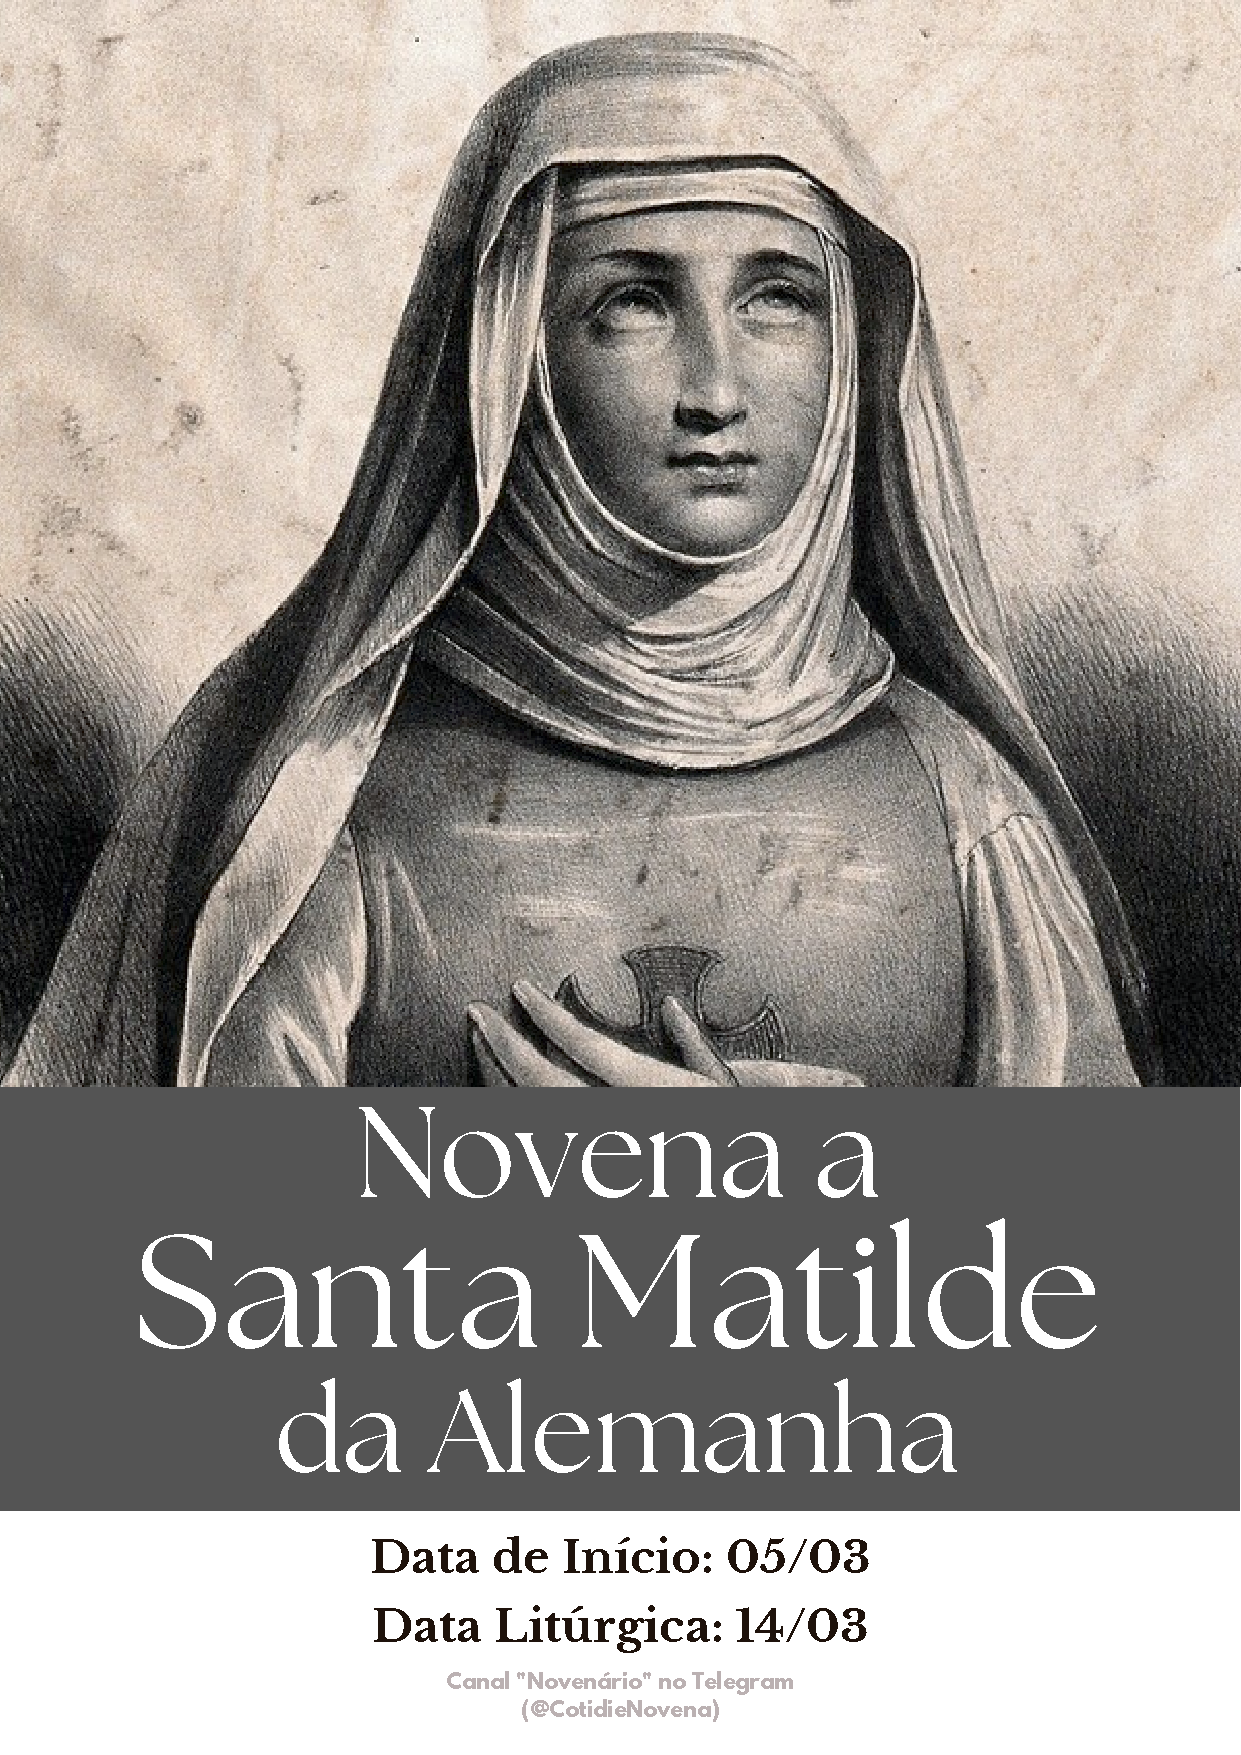
\includepdf[pages=1]{Capa Santa Matilde da Alemanha.pdf}

\begin{center}
  {\huge Novena de Santa Matilde da Alemanha}
\end{center}



\noindent\rule{\textwidth}{0.4pt}

\tableofcontents

\thispagestyle{empty}


% --- Origem ---
\newpage
\section{História}

Santa Matilde (ou Matilde de Ringelheim) foi uma rainha da Germânia conhecida pela piedade, caridade e devoção à Igreja. Esposa do rei Henrique I da Germânia e mãe do imperador Otão I, destacou-se pelo amor aos pobres, pela construção de igrejas e mosteiros e pela vida de oração. Após a morte do marido, enfrentou provações dentro da própria família, mas manteve-se firme na fé. Foi canonizada pela Igreja e é venerada como exemplo de humildade e serviço cristão.

\subsection{Origens e casamento com Henrique I}

Matilde nasceu por volta do ano 895 no seio de uma família nobre saxónica. Foi educada no mosteiro de Herford, onde recebeu uma formação cristã sólida, aprendendo desde cedo a importância da oração e da caridade. Casou-se com Henrique, duque da Saxónia, que mais tarde se tornaria Henrique I, o Passarinheiro, rei da Germânia e fundador da dinastia otoniana. O casal teve cinco filhos, incluindo Otão I, o Grande, que viria a ser o primeiro imperador do Sacro Império Romano-Germânico.

Matilde não se limitou ao papel de rainha consorte. A sua influência foi notável na corte, onde incentivou a justiça e a assistência aos mais necessitados. Era conhecida pela generosidade e pelo profundo espírito cristão.

\subsection{Uma rainha de fé e caridade}

Enquanto rainha, Matilde dedicou-se intensamente a ajudar os pobres e doentes. Fundou hospitais, igrejas e mosteiros, tornando-se protetora das comunidades religiosas. A sua fé era tão profunda que, apesar de viver no palácio, adotava um estilo de vida simples e passava horas em oração.

Entre os mosteiros que ajudou a fundar, destaca-se o de Quedlimburgo, onde mais tarde viveria os últimos anos da sua vida. Apesar das responsabilidades políticas e familiares, nunca deixou de demonstrar humildade e desapego aos bens materiais.

\subsection{Conflitos familiares e exílio}

Após a morte do rei Henrique I, em 936, Matilde viu-se envolvida num conflito entre os seus filhos Otão I e Henrique, que disputavam o trono. Foi acusada de desperdiçar os bens da coroa com as suas obras de caridade e forçada ao exílio. Aceitou esta humilhação com paciência e fé, refugiando-se nos mosteiros que fundara. No entanto, mais tarde foi reconciliada com os filhos e readmitida na corte.

\subsection{Últimos anos e morte}

Nos últimos anos de vida, Matilde retirou-se para o Mosteiro de Quedlimburgo, dedicando-se inteiramente à oração e à vida monástica. Faleceu a 14 de março de 968 e foi sepultada ao lado do marido em Quedlimburgo. Pouco tempo após a morte, passou a ser venerada como santa, devido à sua caridade, humildade e dedicação à fé.

Santa Matilde foi canonizada e tornou-se um modelo de santidade para rainhas e governantes cristãos. A sua festa litúrgica é celebrada a 14 de março. É invocada como padroeira das viúvas e das famílias numerosas, bem como um exemplo de paciência nas provações e de caridade cristã.

\subsection{Conclusão}

Santa Matilde foi uma mulher que soube equilibrar as responsabilidades da realeza com uma profunda espiritualidade. Enfrentou desafios familiares e políticos, mas nunca perdeu a fé nem o compromisso com os mais necessitados. O seu legado vive nas instituições religiosas que fundou e no exemplo de humildade e serviço ao próximo.

% --- Orações Diárias ---
\newpage

\vfill

\section{Orações}

\subsection{Novena de Santa Matilde – 1º dia}

Senhor querido, agradecemos por nos dar Santa Matilde como exemplo de santidade. Ajuda-nos a imitar o amor por Ti que ela demonstrou ao longo de sua vida.

Santa Matilde, de tua infância só sabemos que foste criada por tua avó em uma abadia. Mas sabemos que pelo resto da tua vida após essa infância, rodeada de práticas de oração, serviste fielmente a Deus.

Por favor, leva meus pedidos ao Deus a quem serviste!

Como esposa e mãe, enfrentaste muitas dificuldades. Mas, apesar da morte do teu esposo e das lutas dos teus filhos, fizeste tudo o que podias para servir dignamente a Deus e para ajudar a guiar tua família à virtude.

Roga por mim, para que eu sempre busque servir a Deus em minha vida. Rogai para que eu possa me aproximar de Deus a cada dia.

Por favor, rogai também por \textit{(mencione aqui suas intenções).}

\[\textbf{Pai-Nosso, Ave-Maria, Glória}\]


\subsection{Novena de Santa Matilde – 2º dia}



Senhor querido, agradecemos por nos dar Santa Matilde como exemplo de santidade. Ajuda-nos a imitar a virtude que ela demonstrou ao tentar influenciar o governo de seu esposo para a justiça.

Santa Matilde, te casaste com o duque da Saxônia. Mais tarde, teu marido tornou-se rei do reino dos francos orientais. Embora tu mesma tivesses pouco poder, fizeste todo o possível para influenciar o reinado do teu esposo.

Por favor, faze tudo o que puderes para levar minhas súplicas ao trono de Deus!

Tentaste influenciar teu esposo para que exercesse seu domínio sobre os súditos com justiça. Trabalhaste por essa justiça por amor a Deus.

Roga por mim, para que eu faça tudo o que puder para ajudar a influenciar os outros para o bem. Rogai para que eu possa ajudar a guiar os que me rodeiam à santidade em cada oportunidade.

Por favor, rogai também por \textit{(mencione aqui suas intenções).}

\[\textbf{Pai-Nosso, Ave-Maria, Glória}\]


\subsection{Novena de Santa Matilde – 3º dia}



Senhor querido, agradecemos por nos dar Santa Matilde como exemplo de santidade. Ajuda-nos a imitar a devoção por Ti que ela demonstrou em seu constante serviço aos necessitados ao seu redor.

Santa Matilde, ficaste conhecida por teus atos de caridade durante o teu reinado como rainha. Continuaste este serviço caritativo por toda a tua vida, por amor a Deus.

Por favor, continua levando meus pedidos ao trono de Deus!

Foste tão generosa com os pobres ao teu redor que teus filhos adultos começaram a criticar aquilo que consideravam excesso em tuas obras de caridade.

Roga por mim, para que eu seja sempre generoso com os necessitados, por amor a Deus. Roga para que eu esteja sempre disposto a servir a Deus por meio das obras de caridade para com meus irmãos e irmãs em Cristo.

Por favor, roga também por \textit{(mencione aqui suas intenções).}

\[\textbf{Pai-Nosso, Ave-Maria, Glória}\]


\subsection{Novena de Santa Matilde – 4º dia}



Senhor querido, agradecemos por nos dar Santa Matilde como exemplo de santidade. Ajuda-nos a imitar o Teu amor que ela continuou demonstrando nas provações dos conflitos entre seus filhos adultos.

Santa Matilde, te deparaste com muitas dificuldades após a morte do teu marido. Deve ter sido muito doloroso quando teus filhos adultos iniciaram conflitos armados entre si. Apesar deste sofrimento, perseveraste no serviço a Deus.

Por favor, continua levando minhas preces diante de Deus!

Tentaste mediar entre teus filhos enquanto lutavam entre si. Tentaste influenciar teus filhos para que fossem melhores mesmo quando cediam ao vício e à loucura.

Roga por mim, para que eu sempre procure influenciar os que me cercam para a virtude. Rogai para que eu nunca permita que o sofrimento me desanime de servir a Deus de todo o coração.

Por favor, rogai também por \textit{(mencione aqui suas intenções).}

\[\textbf{Pai-Nosso, Ave-Maria, Glória}\]


\subsection{Novena de Santa Matilde – 5º dia}



Senhor querido, agradecemos por nos dar Santa Matilde como exemplo de santidade. Ajuda-nos a imitar a virtude que ela demonstrou em seu desapego das riquezas materiais.

Santa Matilde, foste rainha do reino dos francos orientais. Apesar de tua alta posição temporal, estavas bastante desprendida das riquezas materiais. Ao invés disso, buscaste a recompensa celestial ao usar tuas riquezas para servir a Deus através de obras de caridade.

Por favor, leva minhas intenções ao Deus a quem tentaste servir com tuas riquezas!

Estavas tão desapegada das riquezas materiais que fizeste obras de caridade que outros consideravam extravagantes. Por fim, abriste mão de tua herança para levar uma vida simples.

Roga por mim, para que eu cresça no desapego dos bens materiais. Roga para que eu sempre busque as riquezas celestes antes das riquezas mundanas.

Por favor, roga também por \textit{(mencione aqui suas intenções).}

\[\textbf{Pai-Nosso, Ave-Maria, Glória}\]


\subsection{Novena de Santa Matilde – 6º dia}



Senhor querido, agradecemos por nos dar Santa Matilde como exemplo de santidade. Ajuda-nos a imitar o Teu amor que ela demonstrou ao trabalhar pela paz em seu país e em sua família.

Santa Matilde, deves ter sofrido grande angústia diante do difícil conflito entre teus filhos adultos. Foste incansável em tentar trazer a paz entre eles.

Por favor, faze tudo o que puderes para levar minhas súplicas ao trono de Deus!

Teus filhos trataram uns aos outros e a seus súditos com grande crueldade. Mas tu nunca deixaste de trabalhar pela paz entre eles, mesmo quando era muito difícil.

Roga por mim, para que nenhuma dificuldade me impeça de fazer o que é certo. Roga para que eu nunca permita que as provações me desanimem de servir a Deus o melhor que eu puder.

Por favor, rogai também por \textit{(mencione aqui suas intenções).}

\[\textbf{Pai-Nosso, Ave-Maria, Glória}\]


\subsection{Novena de Santa Matilde – 7º dia}



Senhor querido, agradecemos por nos dar Santa Matilde como exemplo de santidade. Ajuda-nos a imitar a devoção que ela mostrou, trabalhando para fundar conventos e vivendo o final de sua vida como monja.

Santa Matilde, foste esposa e mãe durante muitos anos. Em tua vocação conjugal fizeste tudo para servir a Deus com devoção sem reservas.

Por favor, leva meus pedidos ao Deus a quem serviste de todo o coração!

Trabalhaste para estabelecer muitos conventos em teu país para que outros pudessem servir a Deus na vida religiosa. Perto do fim da vida, escolheste viver tu mesma os dias como religiosa.

Roga por mim, para que eu esteja sempre disposto a servir a Deus como Ele quiser me chamar. Roga para que eu seja um servo de Deus tão devoto quanto foste tu.

Por favor, roga também por \textit{(mencione aqui suas intenções).}

\[\textbf{Pai-Nosso, Ave-Maria, Glória}\]


\subsection{Novena de Santa Matilde – 8º dia}


Senhor querido, agradecemos por nos dar Santa Matilde como exemplo de santidade. Ajuda-nos a imitar o Teu amor que ela demonstrou fundando conventos e escolhendo viver como monja ao final de sua vida.

Santa Matilde, durante tua vida como Rainha do Reino dos Francos Orientais, trabalhaste para fundar muitos conventos em teu país. Depois da morte de teu esposo, continuaste buscando servir a Deus de novas maneiras.

Por favor, continua levando minhas súplicas diante do trono de Deus!

Finalmente começaste a viver no convento que fundaste em Quedlinburgo. Viveste ali o resto de teus dias.

Roga por mim, para que eu sempre possa servir a Deus de todo o coração em minha vida. Roga para que eu nunca hesite em servir a Deus como Ele me pede.

Por favor, roga também por \textit{(mencione aqui suas intenções).}

\[\textbf{Pai-Nosso, Ave-Maria, Glória}\]


\subsection{Novena de Santa Matilde – 9º dia}



Senhor querido, agradecemos por nos dar Santa Matilde como exemplo de santidade. Ajuda-nos a imitar a devoção para Contigo que ela demonstrou ao longo de sua vida, a serviço de Ti e de Tua Igreja.

Santa Matilde, foste esposa, mãe e rainha durante muitos anos. Fizeste todo o possível para servir dignamente a Deus em tua vocação conjugal e para influenciar positivamente aqueles que te rodeavam.

Continua sempre fazendo tudo o que puderes para levar minhas súplicas diante do trono de Deus!

Fundaste muitos conventos e um mosteiro, e finalmente começaste a viver como religiosa em um desses conventos. Viveste servindo a Deus como monja até tua morte.

Roga por mim, para que eu esteja sempre disposto a servir a Deus e à Sua Igreja de todas as formas possíveis. Roga para que eu nunca me canse de buscar cumprir a vontade de Deus.

Por favor, roga também por \textit{(mencione aqui suas intenções).}

\[\textbf{Pai-Nosso, Ave-Maria, Glória}\]



\vfill

\begin{center}
\subsection*{Fontes:}
Adaptado de: {\color{blue} \underline{\href{https://larutadelavirgendeguadalupe.com/novena-de-santa-matilde/}{La Ruta de La Virgen de Guadalupe}} e {\color{blue} \underline{\href{https://youtube.com/playlist?list=PLN7jQwkJvdQoCTF1o4mfX_l-SMaw4goe0&si=srrIsdAAgNtQvnvw}{Canal A Oração dos Santos}}}}


\end{center}
\end{document}
